
\documentclass[a4paper,12pt]{article}

\usepackage{amsmath}
\usepackage[english]{babel}
\usepackage[margin=1in]{geometry}
\usepackage{graphicx}
\usepackage{listings}

\lstset{tabsize=3, basicstyle=\ttfamily\small, commentstyle=\itshape\rmfamily, numbers=left, numberstyle=\tiny, language=java,moredelim=[il][\sffamily]{?},mathescape=true,showspaces=false,showstringspaces=false,columns=fullflexible,xleftmargin=5pt,escapeinside={(@}{@)}, morekeywords=[1]{let,if,then,else}}
\lstloadlanguages{Java, Haskell}

\newcommand{\kwa}[1]{\mathtt{#1}}
\newcommand{\kw}[1]{\mathtt{#1}~}

\begin{document}



\title{COMP261 Tutorial 2: Tries \\ 21/03/2017}
\date{}
\maketitle

\section{Extension Retrieval}

We are using a Trie in assignment 1 to solve the following problem: given a collection of strings and a prefix P, find those words in the collection that have P as a prefix. For example, those words in $\{ ``sap'', ``soma'', ``soul'', ``slat'' \}$ which extend the prefix $''so''$ are $\{ ``soma'', ``soul''\}$. So we can talk about the complexity of this problem, let us introduce the following variables:

\begin{itemize}
	\item $N$: the number of strings in our collection.
	\item $M$: the maximum length of a string in our collection.
	\item $P$: the length of the prefix whose extensions we want to find.
	\item $L$: the size of the ``language'' of the strings. Characters in the strings are drawn from the language.
\end{itemize}

\noindent
Often we'll think of the language as being fixed. For assignment 1, the language is something like $\{ `A' .. `Z', `a' .. `z' \}$ along with hyphen and space (because a road name can have any of thsese characters). Another language might be $\{ A, C, G, T\}$ --- in bioinformatics, strings of these characters represent DNA molecules.

\section{Finding Extensions With Sets}

To motivate the benefit of Tries, let's imagine how the extension retrieval problem might be solved when the strings are stored in a (hasH0 set. Here are some relevant complexities:

\begin{itemize}
	\item Space: $\mathcal{O}(N \cdot M)$ --- the set stores $N$ strings, and each has length $\mathcal{O}(M)$.
	\item Add: $\mathcal{O}(M)$ --- usually we think of hashing as an $\mathcal{O}(1)$ procedure, but in this case we're also interested in the size of the items being stored. The strings in the set have size $\mathcal{O}(M)$. A typical hash function for strings would have to consider each of the characters in the string --- hence, adding is $\mathcal{O}(M)$. 
	\item Contains: $\mathcal{O}(M)$ --- for similar reasons to add.
\end{itemize}

\noindent
Here is an algorithm for finding all extensions to a given prefix in a (hash) set of strings.

\begin{lstlisting}
find_extensions(set, prefix) {
   extensions = []
   for (string $\in$ set) {
      if (string.startsWith(prefix)) {
         extensions.add(string)
      }
   }
   return extensions
}
\end{lstlisting}

\noindent
The algorithm works by iterating over each string in the collection and adding those which start with $\kwa{prefix}$ into a list. The list is returned at the end. Checking if a string begins with $\kwa{prefix}$ can be done in $\mathcal{O}(P)$ time. This is done once per string, and there are $\mathcal{O}(N)$ strings in the set --- hence the running time is $\mathcal{O}(N \cdot P)$.

\section{Tries}

If the strings are stored in a Trie we can find the extensions faster (a lot of the time). In a Trie, nodes are marked as being a string or not, and each edge out of the node is labelled with a character. If a node is marked as being a string, then those letters along the path from the root to that node comprise a word in our collection. This approach can save space by storing common prefixes along the same path. To wit: 
~\\~\\
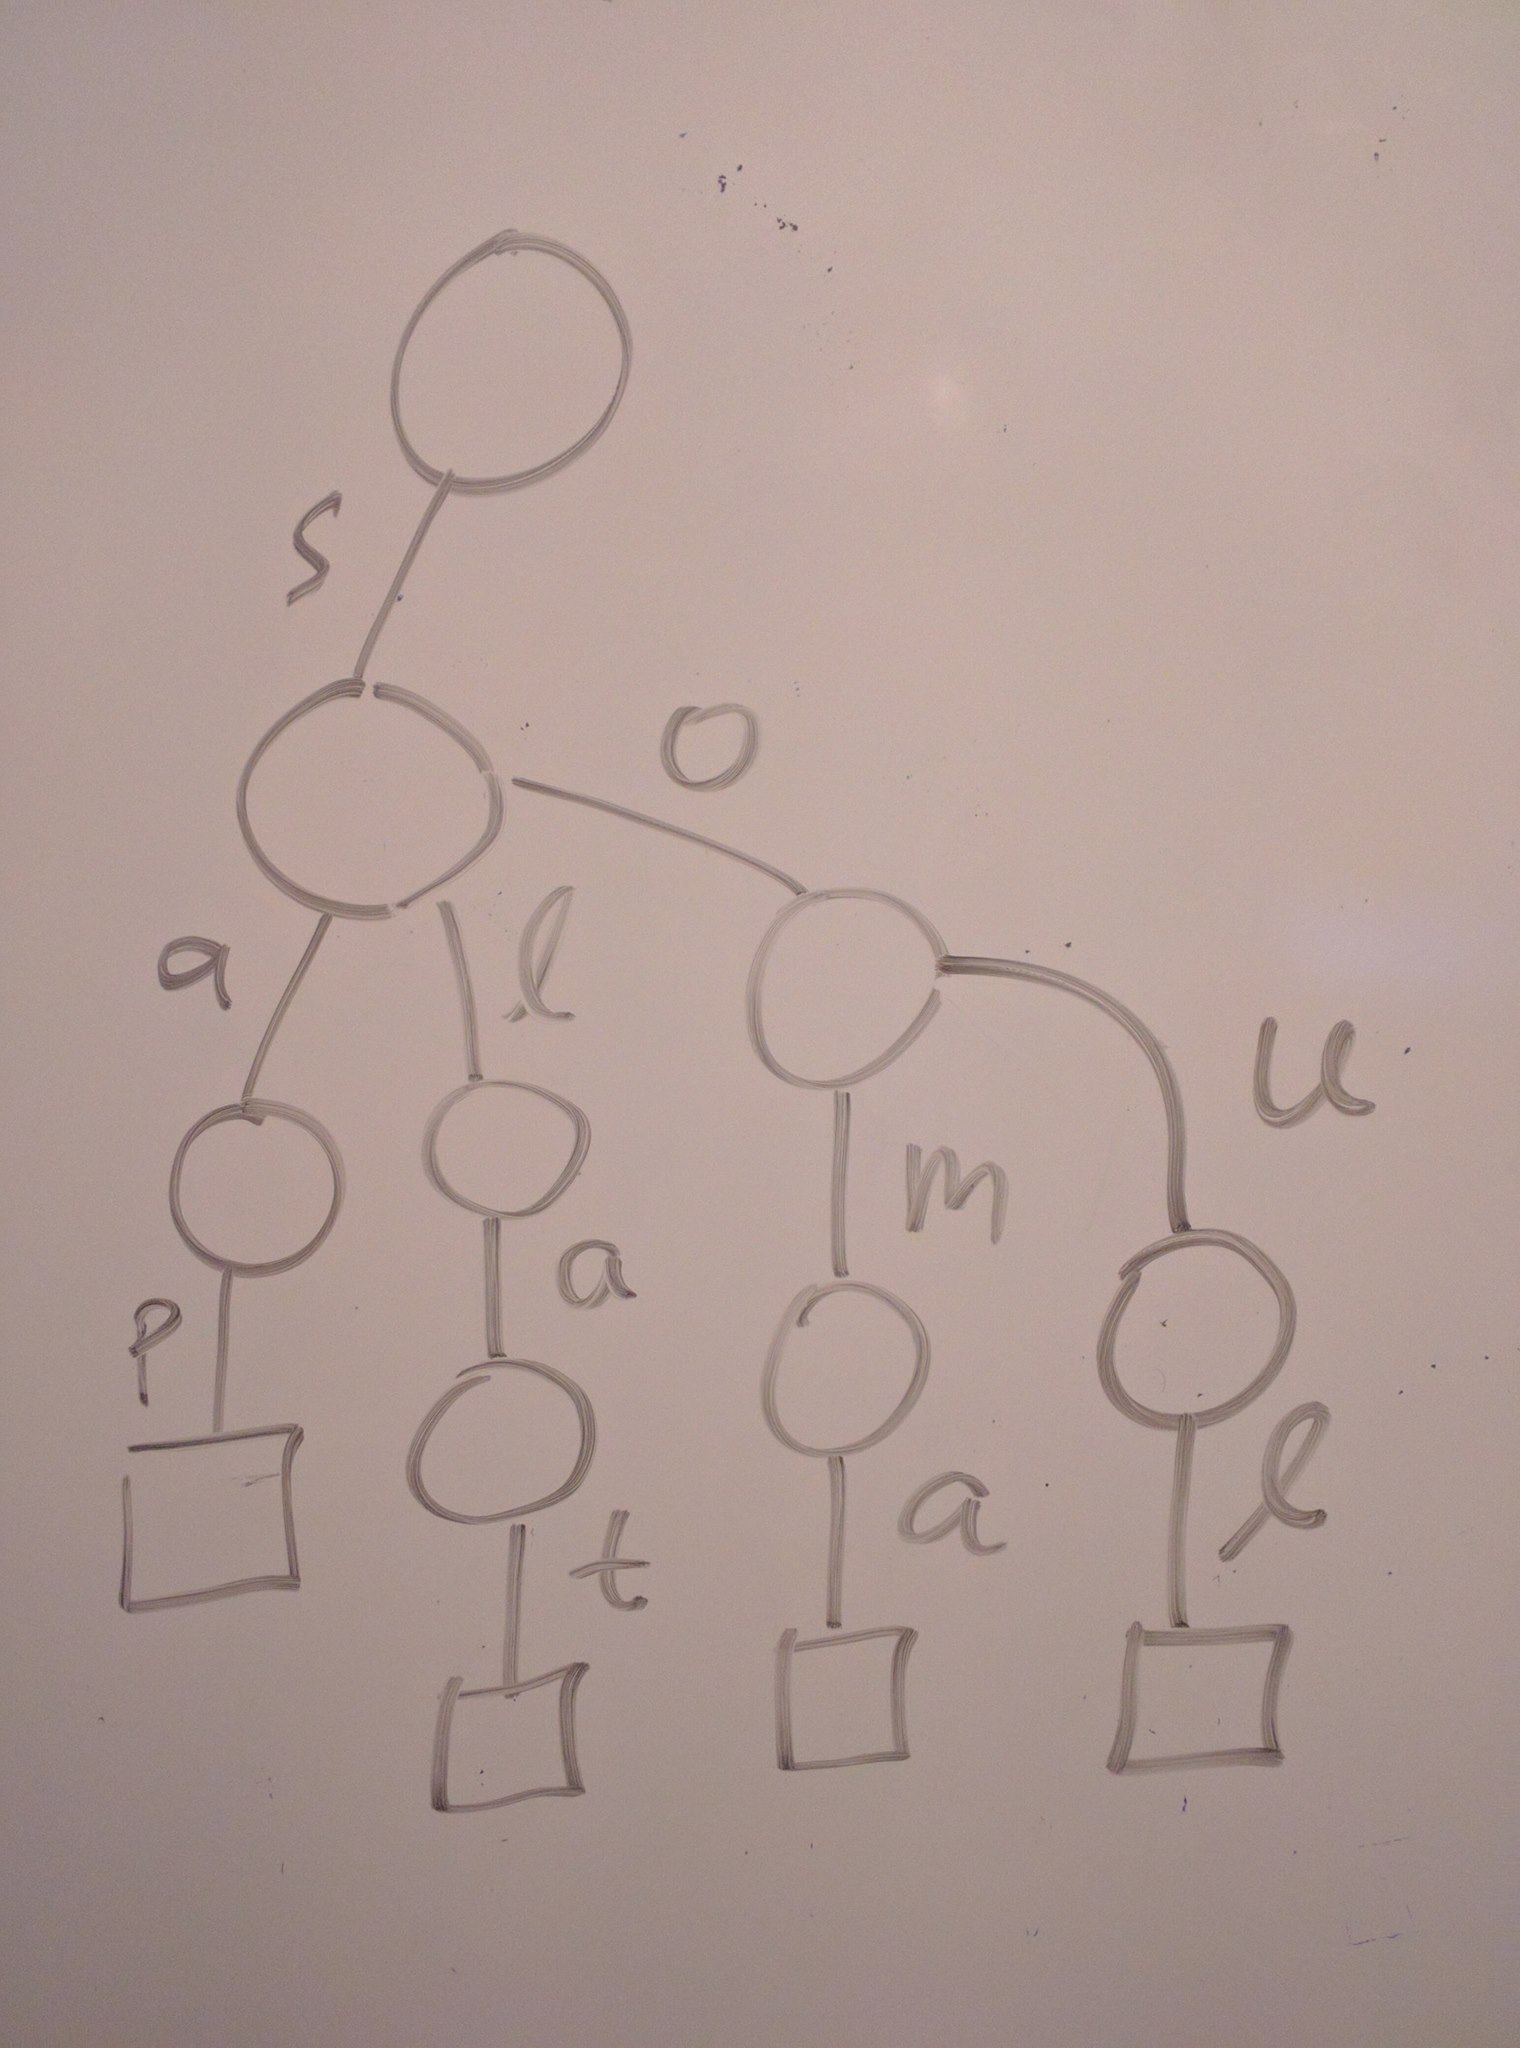
\includegraphics[scale=0.1]{fig_average}
~\\~\\
\noindent
Compare this way of storing things with the set $\{ ``sap'', ``soma'', ``soul'', ``slat'' \}$ --- the $''so''$ prefix in $''soma$ and $''soul''$ is stored twice. In a Trie, they're stored once. In the situation where every string in the collection if a prefix of the longest string, the complexity of the Trie is $\mathcal{O}(M)$. The Trie containing $\{ ``boo'', ``book'', ``booker'' \}$ illustrates this:

~\\~\\
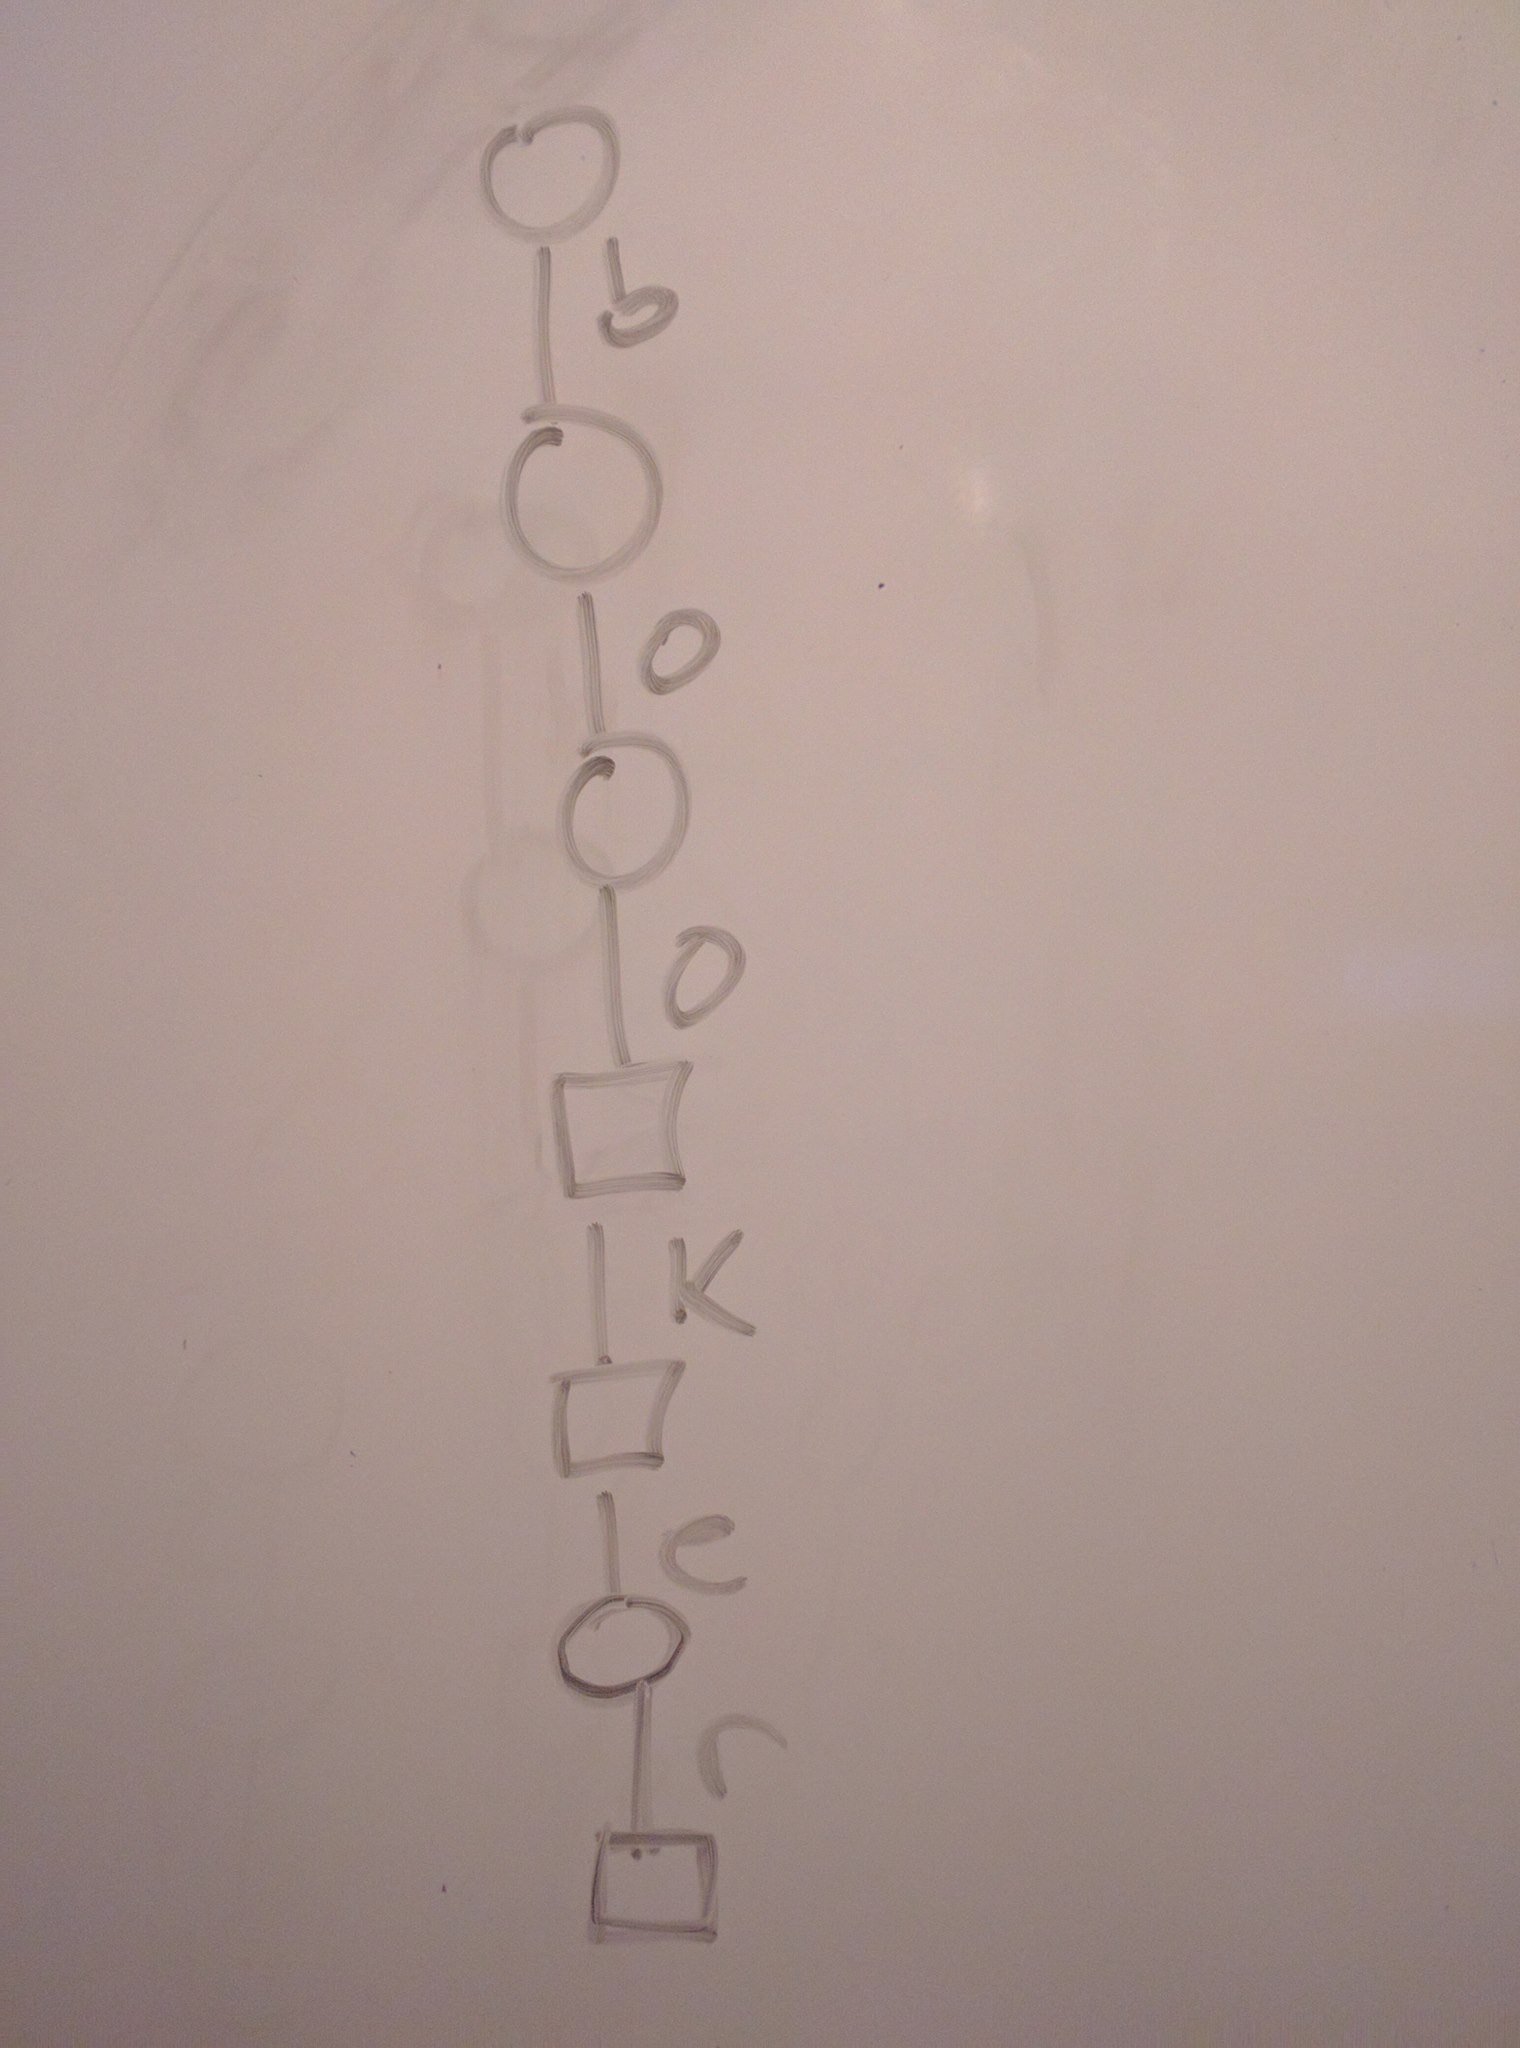
\includegraphics[scale=0.1]{fig_bestcase}
~\\~\\

\noindent
Here are some situations in which a Trie doesn't do so well. When no two strings in the collection have a common prefix, the Trie is at its worst. There will be $\mathcal{O}(N)$ paths, each of length $\mathcal{O}(M)$ --- so the Trie takes up worst case $\mathcal{O}(N \cdot M)$ space. Here's an example of a collection $\{ ``help'', ``kelp'', ``whelp'' \}$ with this behaviour:

~\\~\\
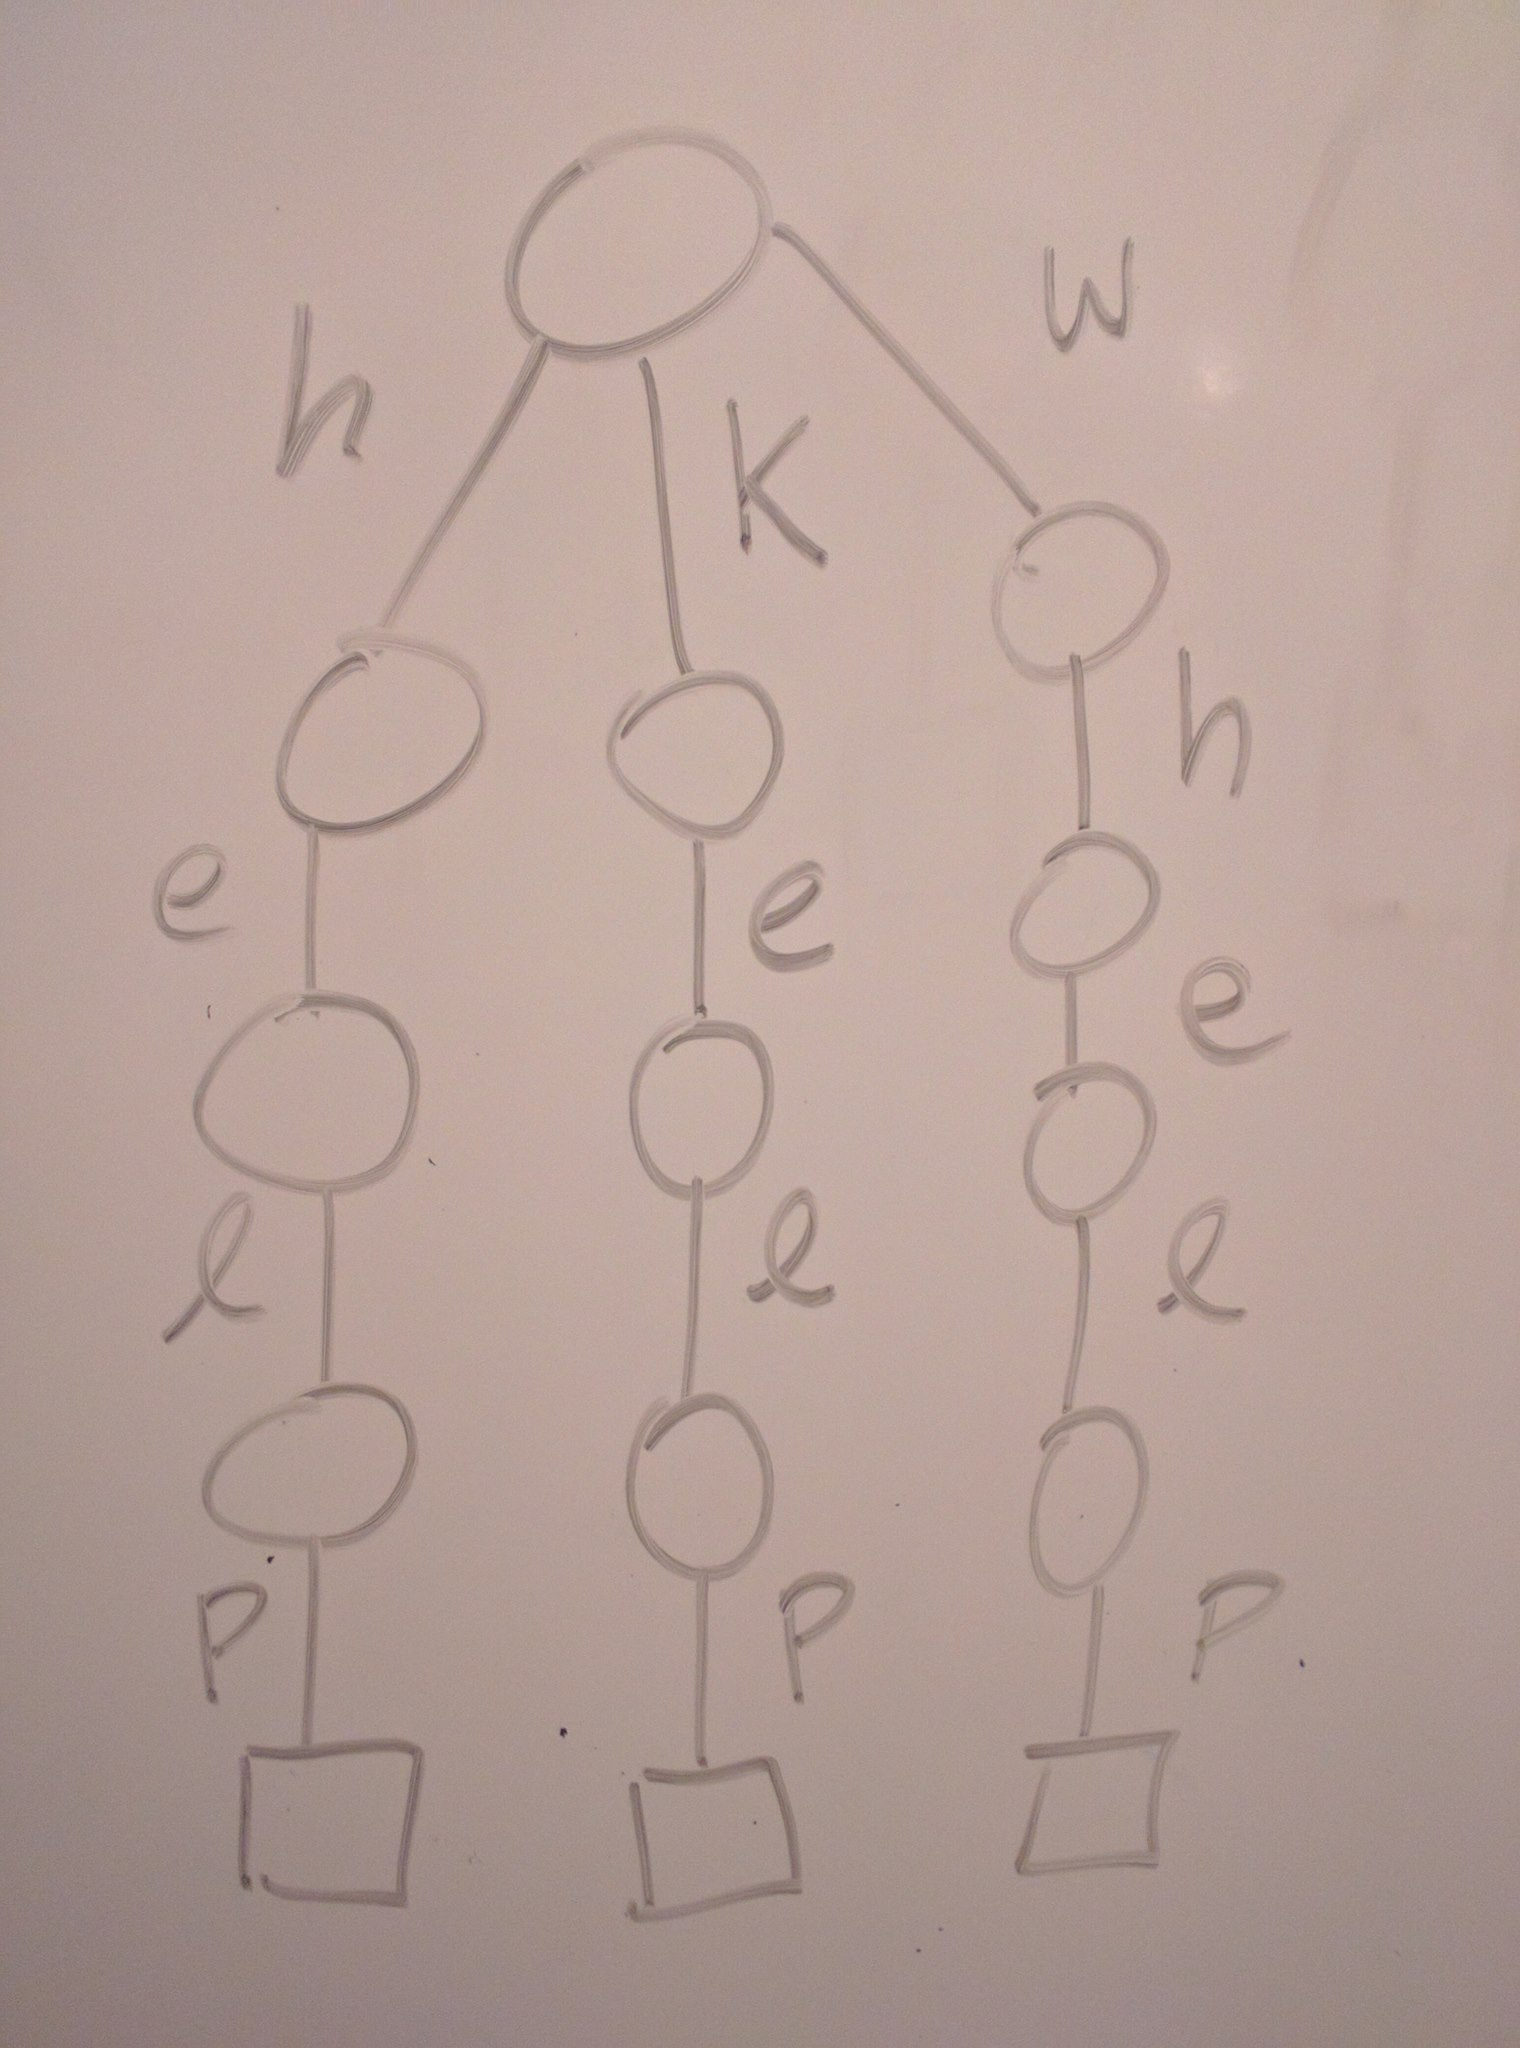
\includegraphics[scale=0.1]{fig_worstcase}
~\\~\\

\noindent
Another situation in which a Trie can be wasteful is when a subtrie contains only one word. In this case, there may be long paths where extra, unnecessary edges could be compressed into a single edge. This is one optimisation of the naïve Trie. The below Trie, containing $\{ ``him'', ``himalayas'' \}$, demonstrates this wastefulness.

~\\~\\
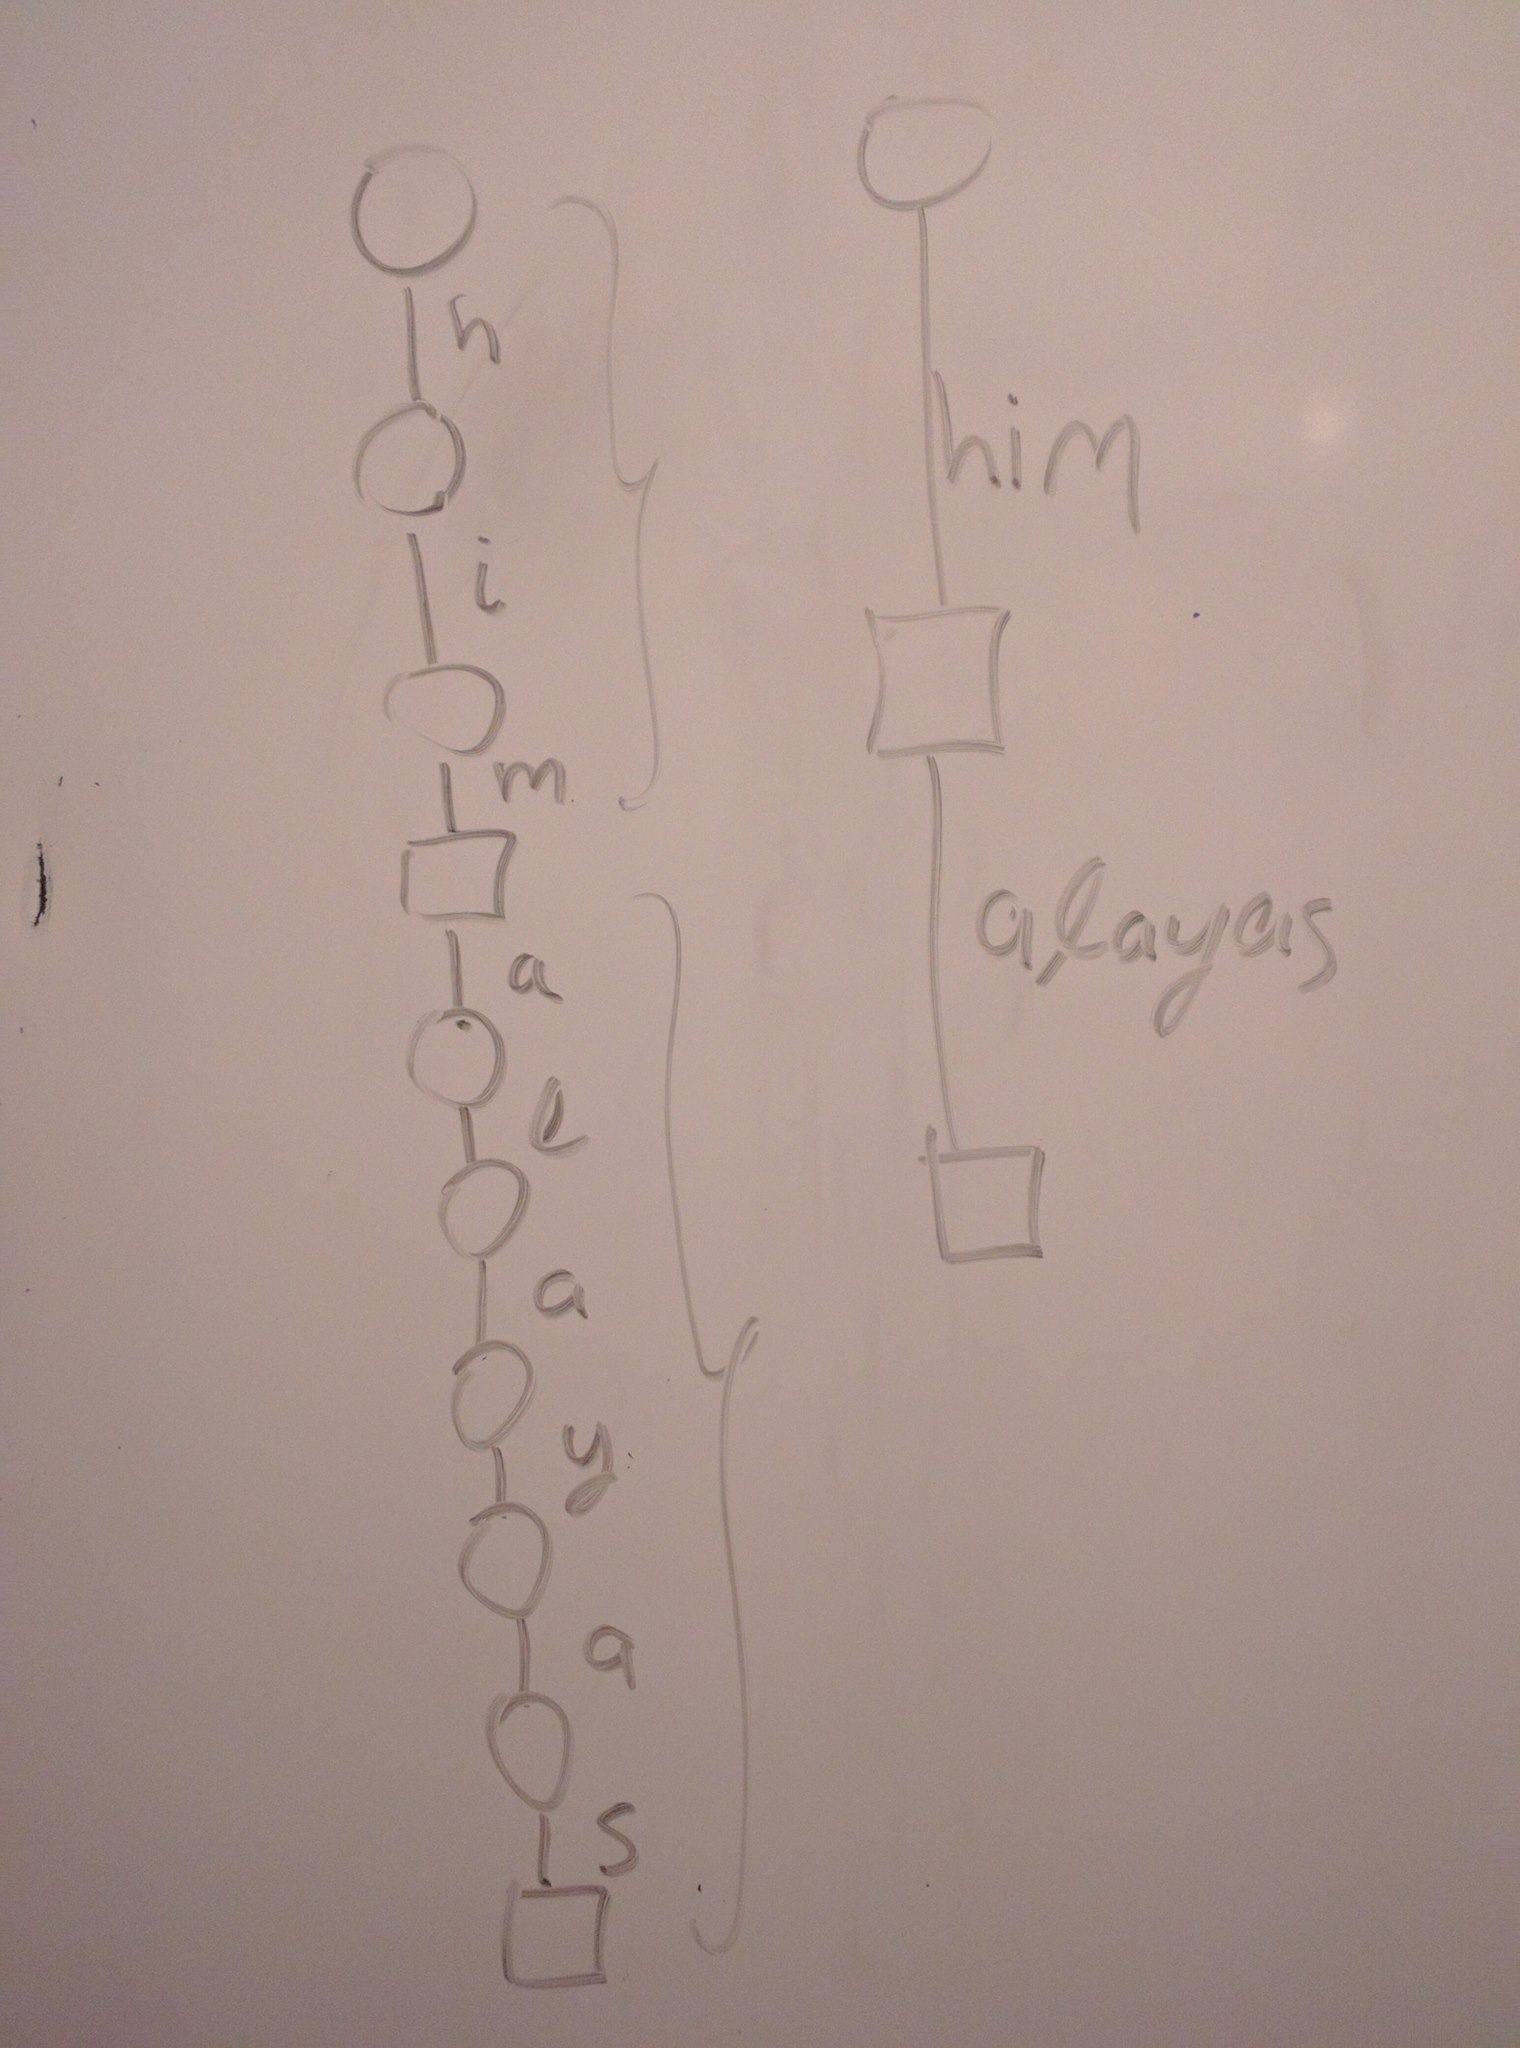
\includegraphics[scale=0.1]{fig_wasteful}
~\\~\\

\noindent
We have seen that the best-case space complexity of a Trie occurs when every string is a prefix of the longest string in this collection --- $\mathcal{O}(M)$. When no two strings share a common prefix, the space complexity is $\mathcal{O}(N \cdot M)$. The other operations of a Trie are the following:

\begin{itemize}
	\item Add: $\mathcal{O}(M)$ --- at worst, you have to create a path of length $\mathcal{O}(M)$.
	\item Contains: $\mathcal{O}(M)$ --- at worst, you have to traverse down a path of length $\mathcal{O}(M)$.
\end{itemize}

\noindent
There are different ways to represent Tries in Java. One way is given below. A ``Trie'' object represents a single node in the Trie. Each Trie has a boolean field determining whether the path from the root to that node comprises a word in the collection. Each Trie also has a map where the keys have type $\kwa{Character}$ and the values have type $\kwa{Trie}$.

\begin{lstlisting}

class Trie {

   private boolean isWord;
   private Map<Character, Trie> kids;

   public void add(String word) { ... }
   public void contains(String word) { ... }

}

\end{lstlisting}


\section{Finding Extensions With Tries}

The algorithm for finding every word in a Trie with a given prefix works in two stages: first, we travese to the node in the Trie where the prefix is stored; second, we collect those words in the subtrie below this node. These will be the words extending the given prefix. An elegant way to do this second part is to return an iterator over the the subtrie where the prefix is contained (in Java terms, Trie would have to implement $\kwa{Iterable<String>}$). A simpler solution --- and the one we'll talk about --- is to collapse that subtrie into a list of strings.

\subsection{Collapse}

Given a Trie of words, $\kwa{collapse}$ returns the words in the Trie as a list. A naïve algorithm is given below. Because we need to remember the path we've taken from the root to the current node, $\kwa{collapse}$ immediately defers to a second version of $\kwa{collapse}$, which remembers the path taken so far. We also pass into each recursive call a list of the words being collected.

\begin{lstlisting}
collapse(trie) {
   wordsInTrie = []
   collapse(trie, ``'', wordsInTrie)
   return wordsInTrie
}
\end{lstlisting}

\begin{lstlisting}
collapse(trie, pathSoFar, wordsInTrie) {
   if (trie.isWord) {
      wordsInTrie.add(pathSoFar)
   }
   for (k $\in$ trie.kids) {
      collapse(trie.kids[k], pathSoFar + k, wordsInTrie)
   }
}
\end{lstlisting}

\noindent
$\kwa{collapse}$ has to iterate over each node in a Trie. At most, this is $\mathcal{O}(N \cdot M)$, so the complexity of $\kwa{collapse}$ is $\mathcal{O}(N \cdot M)$.


\subsection{Extensions}

\noindent
Using $\kwa{collapse}$, we can implement an algorithm for finding every word in a Trie that extends a given prefix. This is done in two steps: first we recurse to the point in the Trie where the prefix is contained, and then we call $\kwa{collapse}$ at that point. If the Trie does not contain the prefix --- meaning no word in the Trie extends that prefix --- then we return the empty list. To figure out how much of the prefix we've matched so far, a second version of $\kwa{extensions}$ takes an index $i$ as an argument. The top-level $\kwa{extensions}$, called by the user, immediately defers to this second version.

\begin{lstlisting}
extensions(trie, prefix) {
   return extensions(trie, prefix, 0)
}
\end{lstlisting}

\begin{lstlisting}
extensions(trie, prefix, index) {
   if (index $\geq$ prefix) {
      extensions = []
      collect(trie, prefix, extensions)
      return extensions
   }
   else {
      charToMatch = prefix[index[
      if (charTomatch $\notin$ trie.kids) {
         return []
      }
      else {
         return extensions(trie.kids[charToMatch], prefix, index+1)
      }
   }
}
\end{lstlisting}

\noindent
There are three cases in the second version of $\kwa{extensions}$. In the first, base case (lines 2-5) we have matched every character in the prefix and found its position in the Trie. All that remains is to $\kwa{collect}$ the words in the subtrie. In the second case (lines 9-10), we are unable to match the next character in the prefix, so the empty list is returned. In the third case (lines 12-13), we match the next character in the prefix and recurse down the tree. \\

\noindent
To understand the complexity of $\kwa{extensions}$, let's analyse the two separate parts of it. In the first part, we must recurse to the point in the Trie containing the prefix. This takes $\mathcal{O}(P)$ operations. Then we must collect on the subtrie below that point. Since the Trie has height at most $\mathcal{O}(M)$ (the maximum length of a word), the subtrie below the location of the prefix in the Trie is going to have height $\mathcal{O}(M-P)$. In the worst case, every word will be in this subtrie. The cost is therefore $\mathcal{O}(P + N \cdot (M - P))$. Note that when the prefix is the empty string, the cost is $\mathcal{O}(N \cdot M)$. When the prefix is a string of length $M$, the cost is $\mathcal{O}(P)$. These are the worst and best cases, respectively.

\end{document}






